\chapter{De la conservation locale aux équations de champ d’Einstein}

Les équations de champ d’Einstein sont assez simples pour tenir sur une seule ligne, mais leur développement en composantes est notoirement pénible. Une métrique comporte de nombreux symboles de Christoffel ; ceux-ci contiennent des dérivées de la métrique ; et le tenseur de courbure contient à la fois des dérivées et des produits de symboles de Christoffel. Avant même d’essayer de résoudre quoi que ce soit, le calcul peut remplir des pages. Pour une métrique donnée, un logiciel de calcul symbolique est souvent le moyen le plus raisonnable de gérer ces calculs.

Les principes sont bien plus simples que les calculs. Nous ne commencerons donc pas par attaquer les équations composante par composante. Nous allons nous demander quelle forme doit avoir l’équation de la gravitation. Le raisonnement part de la théorie de Newton, passe par la conservation locale et aboutit à la découverte de l’unique combinaison de tenseurs de courbure qui peut être égale, de façon cohérente, au flux et à la densité d’énergie et de quantité de mouvement. Dans tout ce chapitre, nous posons \(c=1\).

\section{La double action à l’œuvre en mécanique newtonienne}

La gravitation impose deux consignes complémentaires. Le champ gravitationnel indique à la matière comment se déplacer, tandis que la matière indique au champ gravitationnel quelle forme prendre. Cette double action est déjà visible en mécanique newtonienne.

Soit \(\phi(\mathbf{x},t)\) le potentiel gravitationnel newtonien. Un corps d’épreuve de masse \(m\) subit la force
\begin{equation}
 \mathbf{F}=-m\nabla\phi.
\end{equation}
En combinant cette relation avec \(\mathbf{F}=m\mathbf{a}\), la masse d’épreuve s’élimine :
\begin{equation}
 \mathbf{a}=-\nabla\phi.
\end{equation}
C’est le premier sens de cette interaction. Une fois le champ connu, il indique à tout corps en chute libre comment accélérer, indépendamment de sa masse.

Dans l’autre sens, l’équation de Poisson s’écrit
\begin{equation}
 \nabla^2\phi=4\pi G\rho,
 \qquad
 \nabla^2=
 \frac{\partial^2}{\partial x^2}
 +\frac{\partial^2}{\partial y^2}
 +\frac{\partial^2}{\partial z^2},
 \label{eq:poisson}
\end{equation}
où \(\rho(\mathbf{x},t)\) est la masse par unité de volume. Le facteur \(4\pi\) pourrait être absorbé dans la définition de \(G\), mais il réapparaîtrait simplement ailleurs. L’équation~\eqref{eq:poisson} indique que la distribution de matière est la source du potentiel.

Pour un corps sphérique de masse totale \(M\), la solution à l’extérieur est
\begin{equation}
 \phi(r)=-\frac{GM}{r}.
 \label{eq:newton-potential}
\end{equation}
La densité peut être concentrée près du centre, répartie uniformément ou décroître progressivement vers la surface. La solution extérieure ne dépend que de la symétrie sphérique et de la masse totale. En dehors de la matière,
\(\nabla^2\phi=0\) ; la dérivation de \(1/r\) donne alors la force en raison inverse du carré de la distance. Si seul l’extérieur nous intéresse, nous pouvons réduire la source à un point et utiliser la même expression partout sauf en ce point.

\begin{classroomqa}
\audiencequestion{La densité doit-elle être constante à l’intérieur du corps sphérique, puis tomber brutalement à zéro à sa frontière ?}
\lecturerresponse{Non. Pour ce raisonnement, elle doit être à symétrie sphérique, mais elle n’a pas besoin d’être constante ni de subir une discontinuité. Elle peut décroître progressivement jusqu’à zéro. Aucun de ces détails intérieurs ne modifie le potentiel extérieur, qui ne dépend que de la masse totale.
\lecturetimestamp{00:09:13--00:09:37}}
\end{classroomqa}

Cette formulation en termes de champ paraît plus locale qu’une force directe entre des masses éloignées, mais la gravitation newtonienne comporte toujours une action instantanée à distance. Si la source se déplace, le potentiel newtonien change partout au même instant. La relativité générale doit remplacer cette réponse instantanée, tout comme la loi de force.

\section{Un indice en champ faible, mais pas encore une équation}

La version relativiste de la première consigne est déjà connue : une fois la métrique de l’espace-temps donnée, les particules en chute libre suivent des géodésiques de l’espace-temps. Il nous faut maintenant le remplacement relativiste de l’équation de Poisson, c’est-à-dire la consigne qui indique comment la matière détermine la métrique.

La géométrie de Schwarzschild fournit un indice. Sa composante temporelle est
\begin{equation}
 g_{00}=1-\frac{2GM}{r}.
\end{equation}
En utilisant l’équation~\eqref{eq:newton-potential}, on obtient
\begin{equation}
 g_{00}=1+2\phi.
\end{equation}
Par conséquent,
\begin{equation}
 \nabla^2g_{00}=2\nabla^2\phi=8\pi G\rho.
 \label{eq:weak-mnemonic}
\end{equation}

L’équation~\eqref{eq:weak-mnemonic} doit être prise avec prudence. C’est un aide-mémoire, pas l’équation d’Einstein. Elle fait intervenir une composante privilégiée de la métrique et une source non relativiste. Elle laisse néanmoins entrevoir la structure recherchée : une densité de matière d’un côté et des dérivées secondes de la géométrie de l’autre. C’est l’ébauche du passage de l’équation de Poisson à une équation de champ covariante.

Il faut maintenant examiner de plus près le membre de droite. En unités relativistes, la masse est une énergie ; \(\rho\) doit donc d’abord être comprise comme une densité d’énergie. Mais une densité d’énergie ne constitue pas un objet relativiste complet. Pour voir ce qui l’accompagne, commençons par une grandeur conservée plus simple.

\section{Densité de charge, courant et conservation locale}

Soit \(Q\) la charge électrique et soit \(\sigma\) la densité de charge :
\begin{equation}
 \sigma=\lim_{\Delta V\to0}\frac{\Delta Q}{\Delta V}.
\end{equation}
La densité indique quelle quantité de charge occupe un petit volume spatial à un instant donné. Le courant répond à une autre question. Plaçons dans l’espace une fenêtre orientée infinitésimale et comptons la charge qui la traverse par unité de surface et de temps. Les trois orientations possibles donnent les composantes spatiales du courant \(J^i\).

La comparaison des dimensions est instructive. La densité de charge est la charge divisée par trois longueurs spatiales. Le courant est la charge divisée par deux longueurs spatiales et un intervalle de temps. Lorsque \(c=1\), le temps et la longueur ont les mêmes unités ; la densité et le courant ont donc des dimensions identiques. Ils s’assemblent en un quadrivecteur :
\begin{equation}
 J^\mu=(J^0,J^1,J^2,J^3),
 \qquad J^0=\sigma.
\end{equation}

La conservation de la charge ne signifie pas seulement que la charge totale de l’univers reste constante. Elle est locale. La charge ne peut pas disparaître de la salle de cours pour réapparaître instantanément à Alpha du Centaure. Si elle quitte une région, elle doit traverser la frontière de cette région. Pour une petite boîte, la diminution de la charge à l’intérieur est égale au flux sortant à travers ses parois. Le théorème de Gauss donne
\begin{equation}
 \dot{\sigma}+\nabla\cdot\mathbf{J}=0,
\end{equation}
ou, avec la convention de sommation,
\begin{equation}
 \partial_\mu J^\mu=0.
 \label{eq:charge-continuity}
\end{equation}
En coordonnées courbes, l’équation tensorielle correspondante s’écrit avec une dérivée covariante :
\begin{equation}
 D_\mu J^\mu=0.
\end{equation}
La dérivée covariante n’est pas là pour faire joli. Elle rend l’énoncé valable dans tout système de coordonnées.

\section{Pourquoi l’énergie et la quantité de mouvement nécessitent deux indices}

La charge elle-même est invariante. Des observateurs en mouvement relatif s’accordent sur la charge d’un électron, même s’ils ne s’accordent pas sur la densité de charge ni sur le courant. Un observateur en mouvement voit les volumes contractés par Lorentz et peut observer un courant de charges là où un autre voit des charges au repos. La densité et le courant se mélangent donc lors d’un changement de référentiel, même si la charge totale reste inchangée.

L’énergie et la quantité de mouvement sont plus complexes. Même leurs valeurs totales dépendent du référentiel. Un observateur peut voir une particule au repos, dotée uniquement de son énergie de masse et dépourvue de quantité de mouvement spatiale. Un autre observateur qui passe à côté voit à la fois de l’énergie cinétique et une quantité de mouvement. Ces quatre grandeurs forment le quadrivecteur quantité de mouvement
\begin{equation}
 P^\nu=(P^0,P^1,P^2,P^3),
 \qquad P^0=E.
\end{equation}
Chaque composante \(P^\nu\) est conservée localement. Chacune a donc une densité et un flux. Le premier indice désigne la grandeur conservée ; le second indique s’il s’agit d’une densité ou d’un flux.

Commençons par l’énergie. Sa densité est \(T^{00}\). L’énergie peut aussi traverser une fenêtre : \(T^{0i}\) est donc le flux d’énergie dans la direction \(x^i\). Considérons maintenant la composante \(i\) de la quantité de mouvement. Sa densité est \(T^{i0}\), et son flux dans la direction \(x^j\) est \(T^{ij}\). Avec cette convention :
\begin{itemize}
 \item \(T^{00}\)est la densité d’énergie ;
 \item \(T^{0i}\)est le flux d’énergie dans la direction \(i\) ;
 \item \(T^{i0}\)est la densité de la composante \(i\) de la quantité de mouvement ;
 \item \(T^{ij}\)est le flux de la quantité de mouvement \(i\) à travers une surface de normale \(j\).
\end{itemize}
Le bloc spatial \(T^{ij}\) sera ensuite identifié comme le tenseur des contraintes : ses éléments diagonaux comprennent les pressions, tandis que ses éléments non diagonaux décrivent le cisaillement.

\begin{classroomqa}
\audiencequestion{Lorsque \(T^{m0}(x)\) est appelée la densité de la composante \(m\) de la quantité de mouvement, \(x\) désigne-t-il la composante \(m\) de la position ?}
\lecturerresponse{Non. L’argument \(x\) désigne la position dans l’espace-temps où la densité est évaluée ; il représente l’ensemble des coordonnées. L’indice \(m\) précise quelle composante de la quantité de mouvement est comptée.
\lecturetimestamp{00:41:07--00:41:27}}
\end{classroomqa}

Pour chaque valeur fixée de \(\nu\), la conservation locale donne une équation de continuité :
\begin{equation}
 D_\mu T^{\nu\mu}=0.
 \label{eq:stress-continuity}
\end{equation}
Les quatre valeurs de \(\nu\) donnent une équation pour l’énergie et trois pour la quantité de mouvement. Ensemble, les densités et les flux forment le tenseur énergie-impulsion.

\begin{figure}[htbp]
\centering
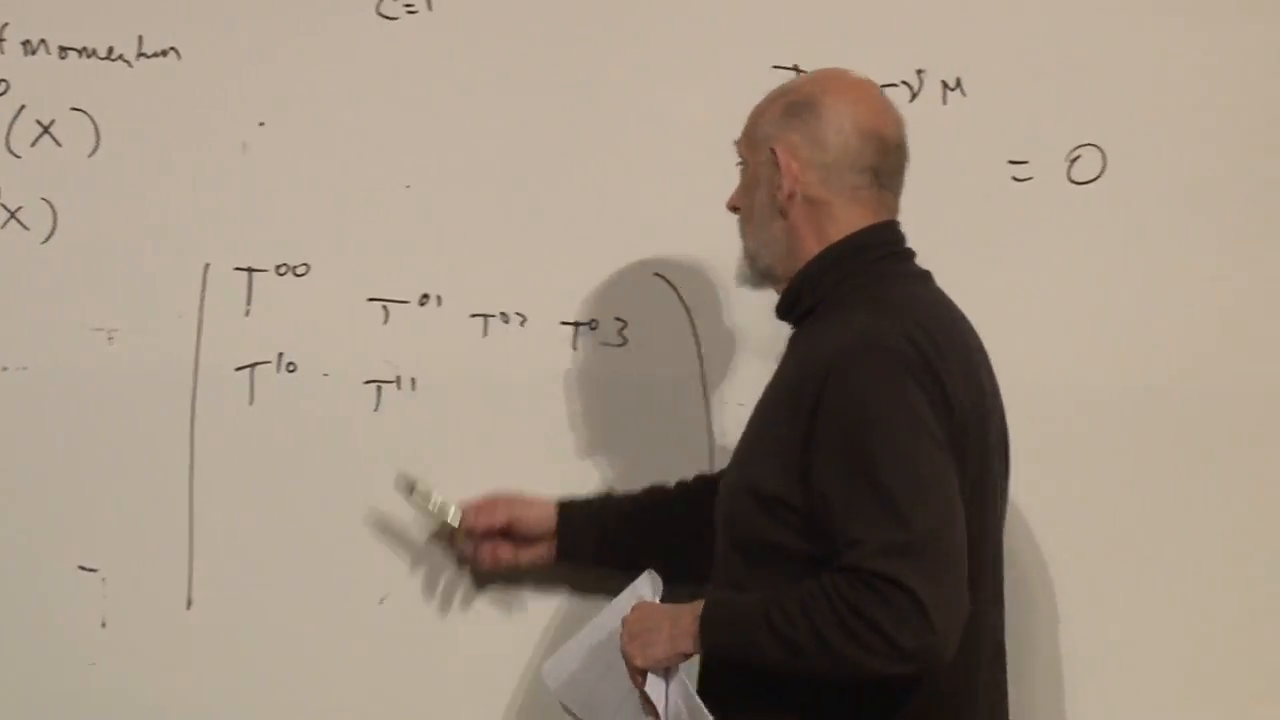
\includegraphics[width=0.84\textwidth]{lecture_09_figure_02.png}
\caption{Le tableau énergie-impulsion en cours d’élaboration au tableau. Le premier indice sélectionne l’énergie ou une composante de la quantité de mouvement ; le second sélectionne la densité ou le flux.}
\lectureframe{00:44:30}
\end{figure}

Le tableau complet est
\begin{equation}
 T^{\mu\nu}=
 \begin{pmatrix}
 T^{00}&T^{01}&T^{02}&T^{03}\\
 T^{10}&T^{11}&T^{12}&T^{13}\\
 T^{20}&T^{21}&T^{22}&T^{23}\\
 T^{30}&T^{31}&T^{32}&T^{33}
 \end{pmatrix}.
\end{equation}
Un autre théorème de la mécanique relativiste et de la théorie des champs implique que le tenseur énergie-impulsion est symétrique :
\begin{equation}
 T^{\mu\nu}=T^{\nu\mu}.
 \label{eq:stress-symmetry}
\end{equation}
En particulier, le flux d’énergie et la densité de quantité de mouvement sont les éléments non diagonaux correspondants, considérés de part et d’autre de la diagonale. La symétrie permet aussi d’écrire l’équation~\eqref{eq:stress-continuity} sous sa forme habituelle :
\begin{equation}
 D_\mu T^{\mu\nu}=0.
 \label{eq:stress-conservation}
\end{equation}

\begin{classroomqa}
\audiencequestion{Pourquoi le tenseur énergie-impulsion a-t-il gagné un indice supplémentaire, alors que le courant de charge n’en nécessitait qu’un ?}
\lecturerresponse{L’indice du courant distingue déjà la densité de la direction du flux. La charge n’a pas besoin d’une étiquette supplémentaire, car la charge conservée est un scalaire. L’énergie et les trois composantes de la quantité de mouvement sont elles-mêmes quatre composantes ; le premier indice précise donc quelle grandeur conservée est considérée, et le second indique s’il s’agit d’une densité ou d’un flux.
\lecturetimestamp{00:45:31--00:47:24}}
\end{classroomqa}

\begin{classroomqa}
\audiencequestion{La matrice \(T^{\mu\nu}\) entière est-elle symétrique, et pas seulement les éléments qui correspondent au flux d’énergie et à la densité de quantité de mouvement ?}
\lecturerresponse{Oui. La matrice entière est symétrique. La signification détaillée de ses éléments spatiaux, notamment la pression et les contraintes, sera développée plus loin.
\lecturetimestamp{00:47:32--00:47:54}}
\end{classroomqa}

La densité d’énergie n’était donc qu’un élément d’un objet plus vaste. La source de la gravitation ne peut pas être de façon cohérente \(T^{00}\) seule ; elle doit faire intervenir le tenseur entier.

\section{Une loi ne peut sélectionner une seule composante}

On peut voir pourquoi une équation tensorielle est nécessaire sans effectuer le moindre calcul de courbure. Supposons que \(A_i\) et \(B_i\) soient des vecteurs et qu’une loi proposée affirme seulement \(A_3=B_3\). Pour que cette égalité soit valable dans tout référentiel tourné, faisons tourner l’axe trois vers l’axe deux. La même loi affirme alors \(A_2=B_2\) ; une autre rotation donne \(A_1=B_1\). Une loi indépendante du référentiel était en réalité l’équation vectorielle
\begin{equation}
 A_i=B_i.
\end{equation}

Les transformations de Lorentz étendent le même raisonnement au temps. Pour que \(A^0=B^0\) soit valable dans tout référentiel inertiel, les transformations de Lorentz mélangent la composante temporelle aux composantes spatiales et imposent l’équation complète \(A^\mu=B^\mu\). Les bonnes lois relativistes égalent des tenseurs de même type.

L’aide-mémoire newtonien isolait \(T^{00}\), mais l’équation relativiste doit prendre la forme
\begin{equation}
 G_{\mu\nu}=8\pi G\,T_{\mu\nu},
 \label{eq:field-schematic}
\end{equation}
où le symbole \(G_{\mu\nu}\) n’est, au départ, qu’un symbole provisoire. Ses propriétés nécessaires sont maintenant claires :
\begin{enumerate}
 \item il doit s’agir d’un tenseur symétrique de rang deux ;
 \item il doit être construit à partir de la métrique, et non de la matière ;
 \item il doit contenir deux dérivées de la métrique ;
 \item sa divergence covariante doit s’annuler.
\end{enumerate}
La dernière condition découle de l’équation~\eqref{eq:stress-conservation}.

\section{À la recherche des tenseurs de courbure}

Les symboles de Christoffel contiennent une dérivée de la métrique :
\begin{equation}
 \Gamma^\sigma_{\tau\nu}
 =
 \frac12 g^{\sigma\delta}
 \left(
 \partial_\tau g_{\delta\nu}
 +\partial_\nu g_{\delta\tau}
 -\partial_\delta g_{\tau\nu}
 \right).
 \label{eq:christoffel}
\end{equation}
Ce ne sont pas des tenseurs ; ils ne peuvent donc pas, à eux seuls, fournir le membre de gauche. Le tenseur de courbure de Riemann est un tenseur :
\begin{equation}
 R^\rho{}_{\sigma\mu\nu}
 =
 \partial_\mu\Gamma^\rho_{\nu\sigma}
 -\partial_\nu\Gamma^\rho_{\mu\sigma}
 +\Gamma^\rho_{\mu\lambda}\Gamma^\lambda_{\nu\sigma}
 -\Gamma^\rho_{\nu\lambda}\Gamma^\lambda_{\mu\sigma}.
 \label{eq:riemann}
\end{equation}
Ses deux premiers termes contiennent des dérivées secondes de la métrique ; les deux derniers contiennent des produits de dérivées premières. C’est précisément l’ordre différentiel suggéré par l’équation newtonienne.

Le problème est la structure des indices. \(R^\rho{}_{\sigma\mu\nu}\) a quatre indices, tandis que \(T_{\mu\nu}\) en a deux. En contractant un indice supérieur et un indice inférieur convenablement choisis, on obtient le tenseur de Ricci,
\begin{equation}
 R_{\mu\nu}=R^\lambda{}_{\mu\lambda\nu}.
 \label{eq:ricci}
\end{equation}
Les autres contractions qui pourraient sembler possibles s’annulent à cause des symétries du tenseur de Riemann ou redonnent le même objet à un signe et une convention d’indices près. Le tenseur de Ricci est symétrique, mais il contient moins d’information que le tenseur de Riemann complet : il peut s’annuler alors que le tenseur de Riemann reste non nul.

\begin{classroomqa}
\audiencequestion{Peut-on simplement contracter deux indices inférieurs du tenseur de Riemann ? Une contraction ne nécessite-t-elle pas un indice covariant et un indice contravariant ?}
\lecturerresponse{Exactement. Il faut d’abord relever un indice à l’aide de la métrique inverse ; de façon équivalente, la contraction doit inclure \(g^{\mu\nu}\). Écrit sous la forme \(R^\lambda{}_{\mu\lambda\nu}\), le couple d’indices supérieur-inférieur requis est explicite.
\lecturetimestamp{01:00:09--01:00:33}}
\end{classroomqa}

En contractant encore une fois le tenseur de Ricci, on obtient le scalaire de courbure,
\begin{equation}
 R=g^{\mu\nu}R_{\mu\nu}.
 \label{eq:ricci-scalar}
\end{equation}
Multiplier ce scalaire par \(g_{\mu\nu}\) donne un autre tenseur symétrique de rang deux. Nous avons donc trouvé deux candidats naturels :
\begin{equation}
 R_{\mu\nu},
 \qquad
 g_{\mu\nu}R.
\end{equation}

\begin{figure}[htbp]
\centering
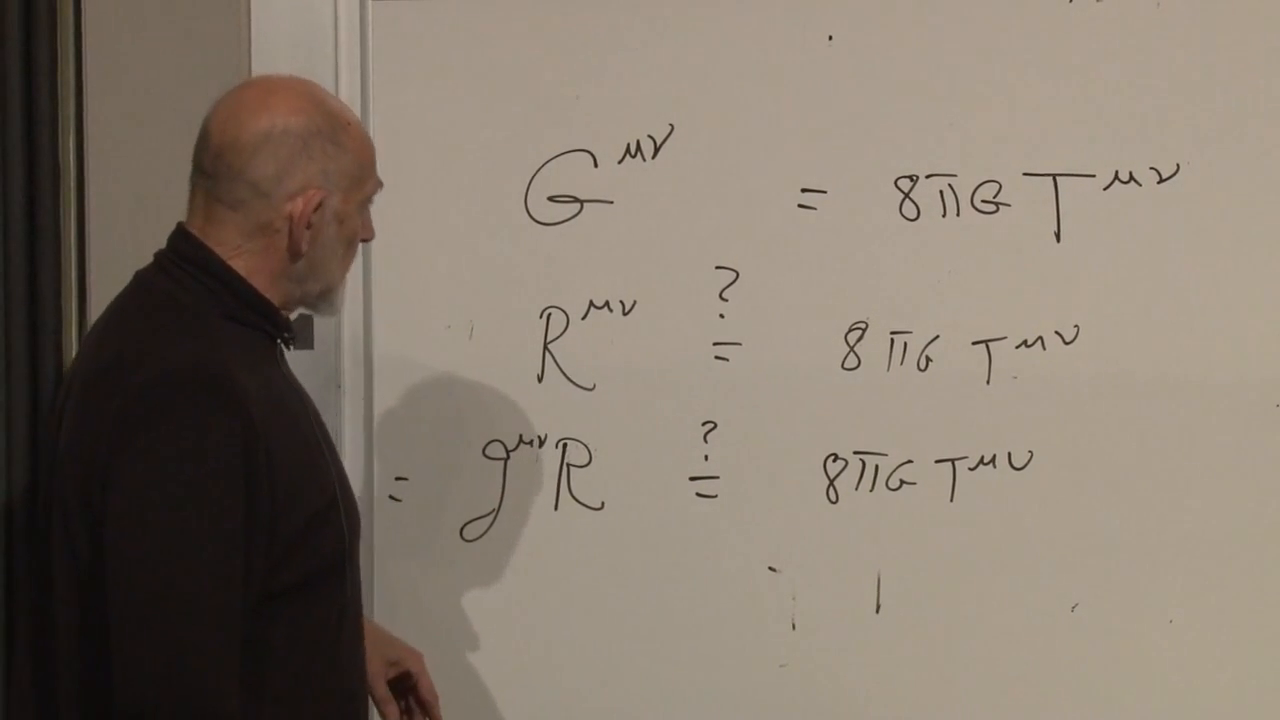
\includegraphics[width=0.78\textwidth]{lecture_09_figure_03.png}
\caption{Les deux tenseurs géométriques envisagés au tableau. À ce stade, leur rang et leur ordre différentiel conviennent tous deux ; chacun est donc accompagné d’un point d’interrogation.}
\lectureframe{01:04:56}
\end{figure}

Les deux possibilités envisagées sont
\begin{align}
 R_{\mu\nu}&\stackrel{?}{=}8\pi G\,T_{\mu\nu},\\
 g_{\mu\nu}R&\stackrel{?}{=}8\pi G\,T_{\mu\nu}.
\end{align}
Aucune ne doit être retenue au seul motif que ses indices conviennent. La conservation permet de les départager.

\section{Le test de la divergence}

Si l’équation~\eqref{eq:field-schematic} est correcte, alors
\begin{equation}
 D_\mu G^{\mu\nu}=0
\end{equation}
doit s’ensuivre identiquement, puisque \(D_\mu T^{\mu\nu}=0\). Commençons par le candidat faisant intervenir le scalaire de courbure. La règle du produit donne
\begin{equation}
 D_\mu\!\left(g^{\mu\nu}R\right)
 =
 \left(D_\mu g^{\mu\nu}\right)R
 +g^{\mu\nu}D_\mu R.
 \label{eq:product-rule}
\end{equation}

\begin{figure}[htbp]
\centering
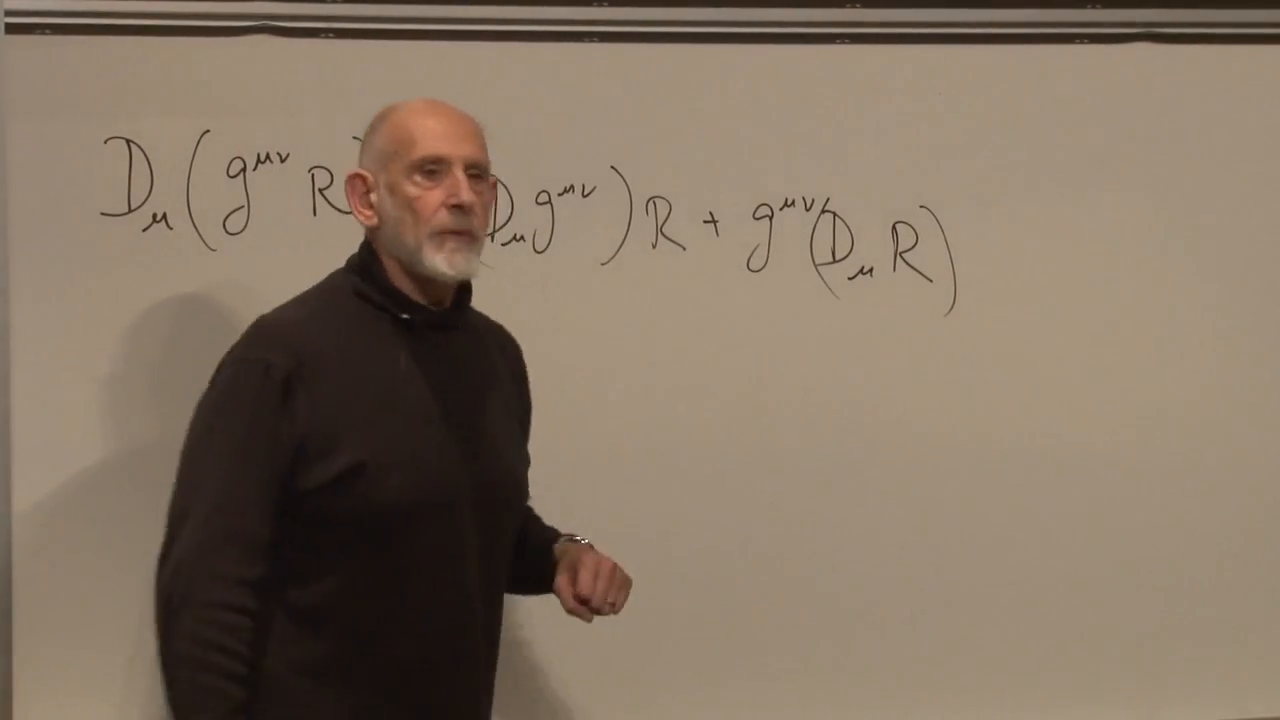
\includegraphics[width=0.84\textwidth]{lecture_09_figure_04.png}
\caption{Application de la règle du produit covariante à \(D_\mu(g^{\mu\nu}R)\).}
\lectureframe{01:07:12}
\end{figure}

La compatibilité métrique s’écrit
\begin{equation}
 D_\mu g^{\alpha\beta}=0.
 \label{eq:metric-compatibility}
\end{equation}
C’est une propriété géométrique indépendante de la connexion de Levi-Civita, et non une conséquence de la conservation de l’énergie-impulsion. Puisque \(R\) est un scalaire, \(D_\mu R=\partial_\mu R\). L’équation~\eqref{eq:product-rule} devient donc
\begin{equation}
 D_\mu(g^{\mu\nu}R)
 =g^{\mu\nu}\partial_\mu R
 =D^\nu R,
\end{equation}
ce qui n’est généralement pas nul. Le candidat \(g^{\mu\nu}R\) échoue.

Le calcul correspondant pour le tenseur de Ricci est un peu plus long. Il aboutit à l’identité de Bianchi contractée,
\begin{equation}
 D_\mu R^{\mu\nu}=\frac12 D^\nu R.
 \label{eq:contracted-bianchi}
\end{equation}
Le tenseur \(R^{\mu\nu}\) échoue donc lui aussi pris isolément. Mais les deux échecs sont dans le rapport précis qui permet une annulation :
\begin{equation}
 D_\mu\left(
 R^{\mu\nu}-\frac12 g^{\mu\nu}R
 \right)=0.
\end{equation}
On obtient ainsi le tenseur d’Einstein,
\begin{equation}
 \boxed{
 G_{\mu\nu}
 =
 R_{\mu\nu}-\frac12 g_{\mu\nu}R
 }.
 \label{eq:einstein-tensor}
\end{equation}

Dans le cadre des hypothèses retenues ici -- à savoir un tenseur local symétrique de rang deux, construit à partir de la métrique et ne contenant pas plus de deux dérivées --, cette combinaison est déterminée à un coefficient global près, avec la possibilité d’ajouter un terme métrique. Ce dernier correspond à la constante cosmologique, qui reviendra vers la fin du cours. Le coefficient devant l’équation~\eqref{eq:einstein-tensor} est fixé en imposant la limite newtonienne.

\begin{classroomqa}
\audiencequestion{Existe-t-il une façon plus directement physique d’obtenir l’équation de champ, plutôt que de proposer des candidats puis de les rejeter à l’aide de l’équation de continuité ?}
\lecturerresponse{La conservation locale est déjà un principe physique : l’énergie et la quantité de mouvement ne peuvent pas disparaître d’une région sans en traverser la frontière. Il existe aussi une dérivation plus condensée, fondée sur un principe d’action pour le champ gravitationnel. La variation de cette action produit la même équation, même si le calcul lui-même n’est pas bref.
\lecturetimestamp{01:17:14--01:18:41}}
\end{classroomqa}

\begin{classroomqa}
\audiencequestion{Un autre tenseur géométrique de rang deux pourrait-il satisfaire la même loi de conservation ? La réponse est-elle d’ordre physique ou mathématique, et Einstein l’aurait-il connue ?}
\lecturerresponse{Dans le cadre des hypothèses de cette construction, la classification est mathématique. Les objets de courbure disponibles avec deux dérivées proviennent du tenseur de Riemann ; les deux candidats de rang deux que nous venons d’examiner couvrent toutes les contractions pertinentes. Il faut néanmoins effectuer un calcul pour trouver la combinaison à divergence nulle. Les principes sont simples, mais gérer les indices et les signes demande du travail.
\lecturetimestamp{01:18:42--01:21:44}}
\end{classroomqa}

\section{L’équation de champ et sa limite newtonienne}

L’équation de champ s’écrit maintenant
\begin{equation}
 \boxed{
 R_{\mu\nu}-\frac12 g_{\mu\nu}R
 =
 8\pi G\,T_{\mu\nu}
 }.
 \label{eq:einstein-equation}
\end{equation}
Le membre de gauche est géométrique ; celui de droite décrit la matière, le rayonnement et leurs flux. Leurs divergences covariantes s’annulent simultanément.

Le facteur \(8\pi G\) n’est pas déterminé par l’argument de divergence. On le détermine en considérant un champ gravitationnel faible et lentement variable, produit par de la matière se déplaçant lentement, puis en exigeant que la composante temporelle reproduise l’équation de Poisson. Dans ce régime, \(T_{00}\simeq\rho\), tandis que les autres composantes sont atténuées par des puissances de \(v/c\). Le membre géométrique se réduit à la structure en dérivées secondes anticipée dans l’équation~\eqref{eq:weak-mnemonic}. L’accord donne exactement la normalisation de l’équation~\eqref{eq:einstein-equation}.

Cette limite explique aussi pourquoi la gravitation newtonienne semble n’avoir pour source que la densité de masse. Dans la théorie complète, chaque composante de \(T_{\mu\nu}\) contribue à la gravitation : la densité d’énergie, le flux d’énergie, la densité de quantité de mouvement, la pression et le cisaillement. Pour la matière ordinaire non relativiste, l’énergie de masse domine. Dans la matière relativiste, le rayonnement ou les systèmes soumis à une forte pression, on ne peut pas négliger les autres composantes.

Le cheminement historique ne fut pas une intuition immédiate et sans effort. Le tenseur de Ricci paraît être le premier candidat évident, et le terme supplémentaire \(-\tfrac12g_{\mu\nu}R\) assure la compatibilité avec la conservation locale. Une fois la structure tensorielle fixée, la limite newtonienne fournit la normalisation.

\section{Ce que la contraction laisse de côté}

\begin{classroomqa}
\audiencequestion{Lorsque les quatre indices du tenseur de Riemann sont contractés pour n’en garder que deux, l’information écartée a-t-elle un contenu physique ?}
\lecturerresponse{Oui. Le tenseur de Ricci ne contient pas toute la courbure de l’espace-temps. Les champs gravitationnels sans source en fournissent les exemples les plus nets : le tenseur de Ricci peut s’annuler alors que la courbure de marée et les ondes gravitationnelles subsistent. La contraction conserve la partie directement liée à l’équation locale de la source, mais pas tous les degrés de liberté du champ gravitationnel.
\lecturetimestamp{01:21:57--01:23:10}}
\end{classroomqa}

L’analogie avec l’électromagnétisme est utile. Les équations de Maxwell admettent des ondes dans une région dépourvue de charge et de courant. De même, l’équation d’Einstein admet une géométrie non triviale dans une région où \(T_{\mu\nu}=0\). Dérivons maintenant l’équation plus simple qui s’y applique.

\section{Le vide signifie Ricci plat, et non plat}

Posons
\begin{equation}
 T_{\mu\nu}=0.
\end{equation}
L’équation~\eqref{eq:einstein-equation} donne alors
\begin{equation}
 R_{\mu\nu}-\frac12g_{\mu\nu}R=0.
 \label{eq:vacuum-einstein}
\end{equation}
Contractons avec \(g^{\mu\nu}\). Comme
\begin{equation}
 g^{\mu\nu}g_{\mu\nu}
 =\delta^\mu{}_\mu=4
\end{equation}
dans un espace-temps à quatre dimensions, la trace est
\begin{equation}
 R-\frac12(4)R=-R=0.
\end{equation}
Par conséquent,
\begin{equation}
 R=0,
 \qquad
 R_{\mu\nu}=0.
 \label{eq:ricci-flat}
\end{equation}
L’équation de champ dans le vide impose que le tenseur de Ricci soit nul.

Il est essentiel de ne pas remplacer les mots \emph{Ricci plat} par \emph{plat}.
L’extérieur de Schwarzschild ne contient aucune matière en dehors de la singularité centrale, et il satisfait à \(R_{\mu\nu}=0\). Pourtant, son tenseur de Riemann est non nul et les forces de marée sont bien réelles. On peut vérifier que le tenseur de Ricci est nul en calculant à la main tous les symboles de Christoffel et toutes les composantes de courbure, au prix d’un calcul fastidieux, ou en confiant ces calculs à un système de calcul symbolique. À la singularité, les expressions classiques divergent ; partout ailleurs, l’équation du vide est vérifiée.

Les ondes gravitationnelles en fournissent un second exemple. Elles peuvent se propager dans une région sans source tout en transportant une véritable déformation de l’espace-temps. Ainsi,
\begin{equation}
 R_{\mu\nu}=0
 \quad\not\Rightarrow\quad
 R^\rho{}_{\sigma\mu\nu}=0.
\end{equation}

\section{Conserver la source : l’équation de la trace}

Le cours est sur le point de s’achever sur le résultat concernant le vide, mais une personne dans le public demande de refaire la contraction sans éliminer la source.

\begin{classroomqa}
\audiencequestion{Qu’obtient-on si l’on effectue la même contraction en laissant \(T_{\mu\nu}\) dans l’équation ?}
\lecturerresponse{La trace relie directement le scalaire de courbure à la trace du tenseur énergie-impulsion ; en réinjectant cette relation dans l’équation, on obtient une forme équivalente de l’équation de champ faisant intervenir le tenseur de Ricci.
\lecturetimestamp{01:29:28--01:32:20}}
\end{classroomqa}

Définissons
\begin{equation}
 T=g^{\mu\nu}T_{\mu\nu}.
\end{equation}
La trace de l’équation~\eqref{eq:einstein-equation} donne
\begin{align}
 R-\frac12(4)R&=8\pi G\,T,\\
 -R&=8\pi G\,T,
\end{align}
par conséquent,
\begin{equation}
 \boxed{R=-8\pi G\,T}.
 \label{eq:trace-relation}
\end{equation}
En reportant ce résultat dans l’équation de champ, on obtient
\begin{equation}
 \boxed{
 R_{\mu\nu}
 =
 8\pi G
 \left(
 T_{\mu\nu}-\frac12g_{\mu\nu}T
 \right)
 }.
 \label{eq:ricci-form}
\end{equation}

\begin{figure}[htbp]
\centering
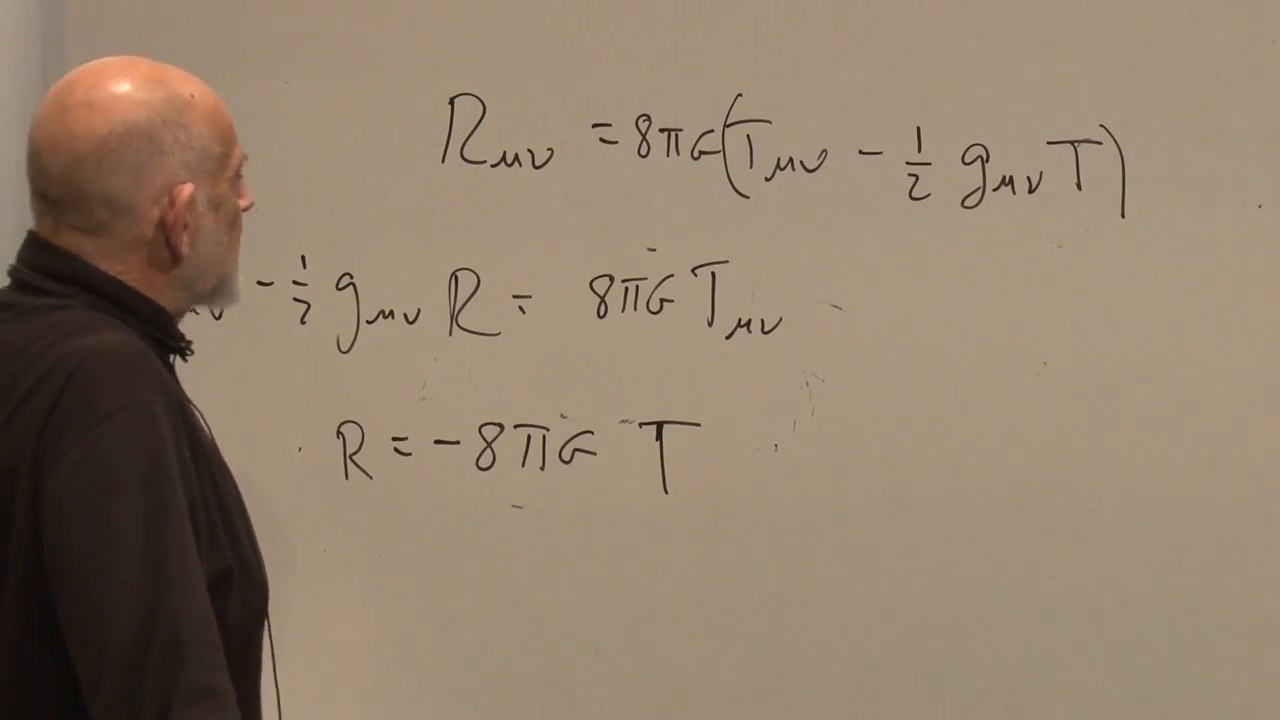
\includegraphics[width=0.82\textwidth]{lecture_09_figure_05.png}
\caption{La relation de trace et la forme équivalente de l’équation d’Einstein faisant intervenir le tenseur de Ricci.}
\lectureframe{01:32:25}
\end{figure}

\begin{classroomqa}
\audiencequestion{Le scalaire \(T\) a-t-il une signification physique ?}
\lecturerresponse{C’est la trace du tenseur énergie-impulsion. Elle s’annule pour le rayonnement électromagnétique ; il en va de même pour un gaz parfait de particules sans masse, comme les photons. La matière massive a généralement une trace non nulle. Par l’intermédiaire de l’équation~\eqref{eq:trace-relation}, cette trace détermine le scalaire de courbure.
\lecturetimestamp{01:32:20--01:33:12}}
\end{classroomqa}

\section{Quelle part de la courbure le tenseur de Ricci retient-il ?}

\begin{classroomqa}
\audiencequestion{Existe-t-il une représentation physique ou géométrique simple du tenseur de Ricci et du scalaire de Ricci, comparable au transport parallèle autour d’une petite boucle pour le tenseur de Riemann ?}
\lecturerresponse{Aucune représentation aussi transparente n’est proposée ici. Le tenseur de Riemann décrit directement la rotation résultant du transport autour d’une petite boucle. Ses contractions sont plus simples algébriquement, mais il est plus difficile de visualiser leur signification géométrique individuelle. Mieux vaut ne pas inventer une représentation trompeuse sous prétexte qu’elle serait commode.
\lecturetimestamp{01:33:14--01:34:13}}
\end{classroomqa}

La quantité d’information perdue lors de la contraction dépend de la dimension. En quatre dimensions, le tenseur de Riemann contient des informations sur la courbure absentes du tenseur de Ricci. En trois dimensions, le tenseur de Riemann est déterminé par le tenseur de Ricci. En deux dimensions, le scalaire de courbure contient toute l’information indépendante sur la courbure. La gravitation en quatre dimensions admet donc des degrés de liberté de courbure sans source, invisibles dans \(R_{\mu\nu}\).

\begin{classroomqa}
\audiencequestion{Si des tenseurs de Riemann différents peuvent avoir le même tenseur de Ricci, comment l’information manquante se manifeste-t-elle physiquement ?}
\lecturerresponse{Une source donnée ne spécifie pas à elle seule toutes les configurations gravitationnelles possibles. Les données aux limites et les données initiales peuvent inclure un rayonnement gravitationnel. Dans l’approximation de champ faible, on peut imaginer partir d’une solution avec source et y ajouter une onde gravitationnelle libre. La théorie non linéaire complète n’autorise pas une superposition arbitraire, mais cet exemple identifie correctement l’information manquante : une courbure qui se propage et n’est pas déterminée localement par \(T_{\mu\nu}\).
\lecturetimestamp{01:37:05--01:38:59}}
\end{classroomqa}

Deux exemples de vide s’accordent maintenant. La géométrie de Schwarzschild présente une courbure de marée à l’extérieur d’une masse. Une onde gravitationnelle transporte une courbure qui se propage librement. Chacune peut satisfaire à \(R_{\mu\nu}=0\) tout en restant non plate.

\section{La constante cosmologique}

\begin{classroomqa}
\audiencequestion{N’y a-t-il pas de facteur d’ajustement supplémentaire, comme une constante cosmologique ?}
\lecturerresponse{Une constante cosmologique est possible. On peut l’écrire du côté géométrique sous la forme d’une constante multipliée par \(g_{\mu\nu}\), ou la déplacer à droite et l’interpréter comme une contribution du vide au tenseur énergie-impulsion. Ces deux descriptions sont la même équation, avec une répartition différente des termes.
\lecturetimestamp{01:39:01--01:40:44}}
\end{classroomqa}

Avec une constante cosmologique, une convention courante consiste à écrire
\begin{equation}
 G_{\mu\nu}+\Lambda g_{\mu\nu}
 =
 8\pi G\,T_{\mu\nu}.
\end{equation}
En déplaçant le terme supplémentaire vers la droite, on définit un tenseur effectif des contraintes du vide,
\begin{equation}
 T_{\mu\nu}^{(\Lambda)}
 =
 -\frac{\Lambda}{8\pi G}g_{\mu\nu}.
\end{equation}
Comme la compatibilité métrique donne \(D_\mu g^{\mu\nu}=0\), le terme supplémentaire est automatiquement compatible avec la loi de conservation. C’est le terme métrique laissé en suspens dans l’affirmation d’unicité précédente.

\section{Mercure et le calcul en champ faible}

\begin{classroomqa}
\audiencequestion{Einstein a-t-il utilisé cette équation pour calculer l’orbite de Mercure, et où peut-on voir comment ce calcul a été effectué ?}
\lecturerresponse{Einstein a travaillé avant que Schwarzschild ne fournisse la solution exacte ; il a plutôt utilisé une approximation à grande distance suffisamment précise du champ extérieur du Soleil. Le rayon du Soleil et l’orbite de Mercure sont très grands par rapport au rayon de Schwarzschild du Soleil, de sorte que les corrections relativistes sont faibles. Il pouvait partir d’une orbite képlérienne et calculer la correction par perturbation. Peu après, Schwarzschild a obtenu la solution extérieure exacte, ce qui a rendu le même calcul systématique.
\lecturetimestamp{01:40:46--01:43:48}}
\end{classroomqa}

La théorie des perturbations consiste exactement en ceci : partir d’un problème déjà résolu, puis calculer l’effet d’une petite correction. La force newtonienne en raison inverse du carré de la distance produit des ellipses képlériennes fermées. La relativité générale ajoute une petite déviation à l’équation radiale newtonienne ; l’ellipse ne se referme donc pas après une révolution et son périhélie avance.

Le cours s’achève sur le caractère singulier des orbites fermées sous l’action d’une force centrale. La force en raison inverse du carré de la distance est exceptionnelle en ce qu’elle produit des orbites képlériennes fermées, sans précession. Plus généralement, le théorème de Bertrand désigne également l’oscillateur harmonique isotrope comme l’autre potentiel central pour lequel toutes les orbites liées sont fermées. La faible correction relativiste supprime cette dégénérescence newtonienne et fait de la précession de Mercure une signature observable de l’équation de champ établie dans ce chapitre.